\section*{Aufgabe 26}
\label{sec:Aufgabe3}

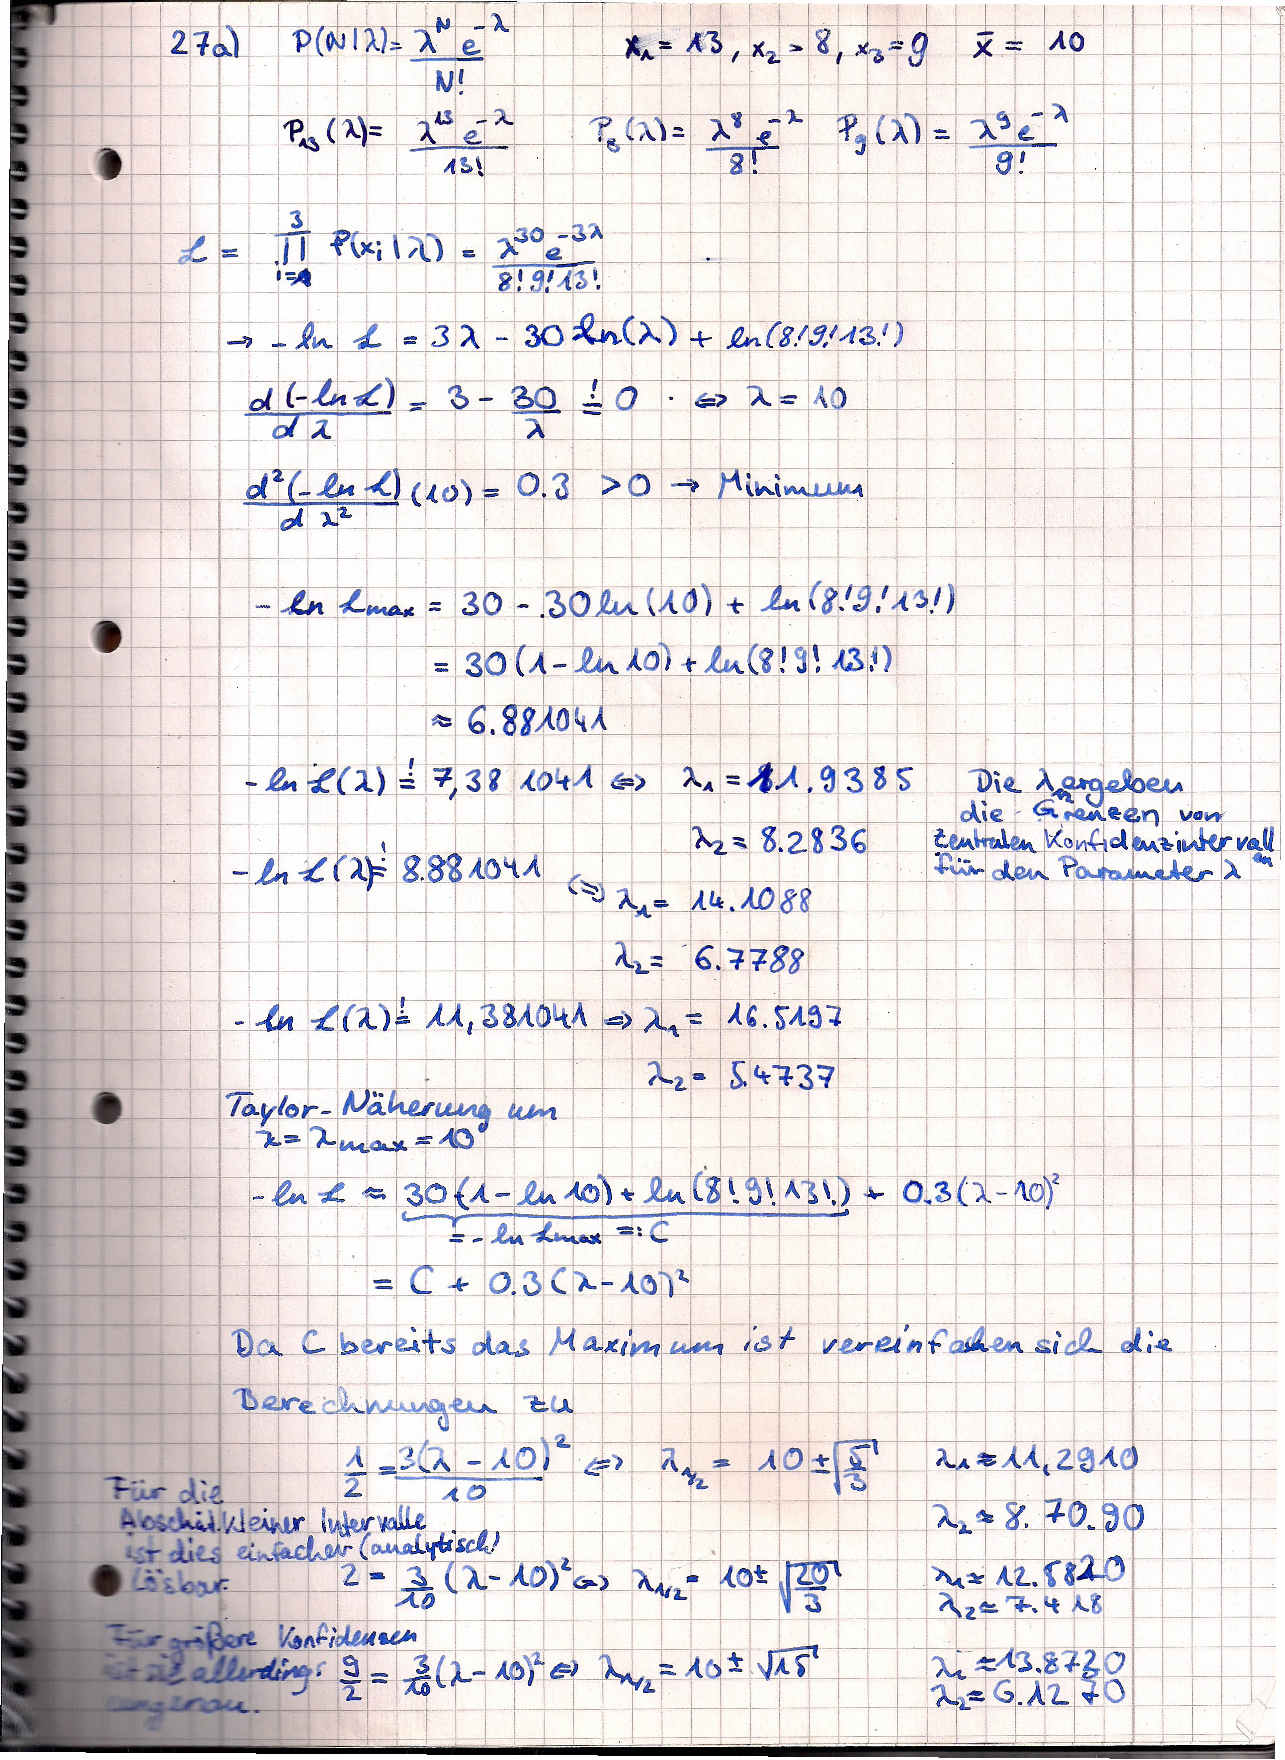
\includepdf[pages=-]{content/images/26.pdf}

\subsection*{a)+d)}
Die exakte negative Log-Likelihood-Funktion, sowie die Taylornäherung in zweiter Ordnung sind in Abbildung \ref{fig:taylor} zu sehen.
Auch wenn sich die Berechnungen der Intervallgrenzen vereinfachen, wird deutlich das für größere Intervalle die Abweichungen sehr deutlich werden.

\begin{figure}
\centering
\includegraphics[width=\textwidth]{build/Likelihood.pdf}
\caption{Log-Likelihood exakt und Taylorentwicklung.}
\label{fig:taylor}
\end{figure}